\let\textcircled=\pgftextcircled
\chapter{Concepts généraux et État de l'art}
\label{chap:background}
\initial{D}\textit{ans ce Chapitre, nous introduisons les informations et les concepts de base nécessaires à la compréhension du travail présenté dans ce document. Il s'agit des notions liées à l'\textbf{extraction intelligente de documents}. Nous passerons ensuite en revue les différentes \textbf{solutions existantes}, leurs limitations et enfin, nous terminerons par un \textbf{Bilan et Positionnement}.}
\vspace{3mm}
\chaptertoc
\newpage
%%%%%%%%%%%%%%%%%%%%%%%%%SECTION GENERALITES%%%%%%%%%%%%%%%%%%%%%%%%%%%%%%%%%%%%%%%%%%%%%%%%%%%%%%%%%
\section{Généralités}
\subsection{Extraction intelligente de documents}
\subsubsection{Définition de l'extraction intelligente de documents}

\textbf{L'extraction intelligente de documents } (\textit{Intelligent Document Processing}  IDP) désigne l'ensemble des technologies permettant de capturer, classifier et extraire automatiquement des informations pertinentes à partir de documents non structurés ou semi-structurés, en utilisant des algorithmes informatiques \cite{gantz2012digital, borchmann2021due}. Cette opération s'appuie sur des technologies d'Intelligence Artificielle qui dépassent la simple lecture de caractères, en analysant la structure spatiale, le contexte sémantique et les relations entre les éléments du document pour en extraire des données exploitables.

Exemple :
Document source : une facture numérisée au format PDF contenant des champs tels que « Montant Total : 1 500 000 FCFA », « Date : 15/03/2025 », « Fournisseur : SABC Cameroun ».
Sortie structurée : un fichier JSON contenant les paires clé-valeur extraites automatiquement.

Parmi les outils populaires intégrant cette technologie, on trouve AWS Textract, Azure Document Intelligence, Google Document AI, qui offrent des services d'extraction documentaire accessibles via API.

La figure~\ref{fig:idp-overview} présente une illustration du processus global d'extraction intelligente de documents.
\begin{figure}[H]
    \centering
    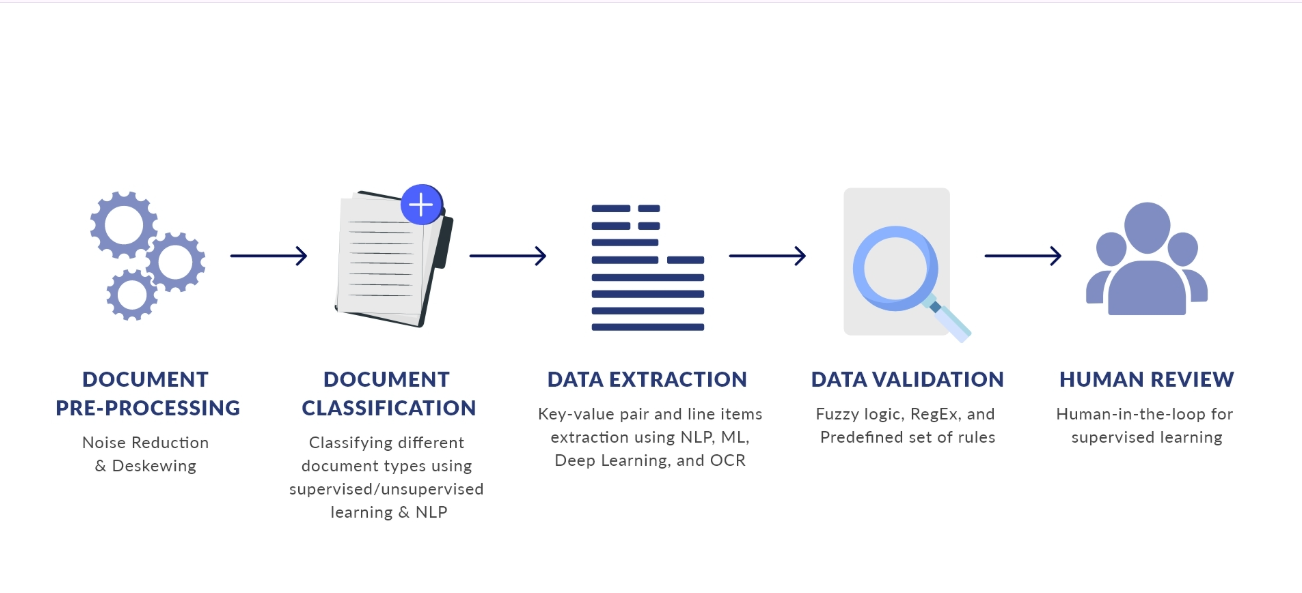
\includegraphics[scale=.6]{chapters/fig/idp_overview.png}
    \caption{\it Principe fonctionnel de l'extraction intelligente de documents}
    \cite{borchmann2021due}
    \label{fig:idp-overview}
\end{figure}


\subsubsection{Méthodes d'extraction documentaire}

Plusieurs approches coexistent pour réaliser l'extraction automatique d'informations à partir de documents, chacune reposant sur des principes et technologies différents \cite{smith2007tesseract, xu2020layoutlm} :

\begin{itemize}[label=\ding{42}, font=\large \color{darkgray}]
\item Extraction par correspondance de templates (\textit{Template Matching}) :
Cette méthode utilise des modèles spatiaux prédéfinis manuellement par des experts pour localiser et extraire les champs d'intérêt dans les documents. Bien qu'offrant une précision exceptionnelle ($>$98\%) sur les documents à structure fixe, elle reste rigide face aux variations de mise en page \cite{lu2003document}.

\item Extraction basée sur la reconnaissance optique de caractères (OCR) :
Elle s'appuie sur des moteurs de reconnaissance de caractères qui convertissent les images de documents en texte exploitable. L'OCR traite les documents en deux étapes détection de texte puis reconnaissance de caractères  et offre une flexibilité élevée face à la diversité des formats. Les moteurs modernes comme Tesseract 5.5.3 atteignent une précision d'environ 92\% sur le texte imprimé standard \cite{smith2007tesseract}.

\item Extraction par apprentissage automatique et IA :
Basée sur des architectures de réseaux de neurones profonds, cette approche est la plus récente et avancée. Elle traite les documents de manière end-to-end en combinant compréhension visuelle et sémantique, ce qui permet une extraction plus robuste face aux variations de layout. L'approche par IA est devenue la norme dominante pour le traitement de documents complexes \cite{xu2020layoutlm, huang2022layoutlmv3}.
\end{itemize}

Dans la suite de ce travail, l'accent sera mis sur une approche hybride combinant template matching et OCR, en raison de l'équilibre qu'elle offre entre précision, coût computationnel et adaptabilité aux documents d'entreprise.


\subsection{Extraction documentaire par correspondance de templates}

L'extraction documentaire par correspondance de templates constitue l'une des méthodes les plus anciennes et les plus fiables pour le traitement de documents à structure connue. On distingue principalement trois familles d'algorithmes selon le type de caractéristiques exploitées.

\subsubsection{Template Matching par projections de blocs composants}

La figure~\ref{fig:template-matching} montre le processus de correspondance spatiale entre un document d'entrée et les templates stockés : extraction de caractéristiques, comparaison avec les templates, sélection du template le plus similaire.

\begin{figure}[H]
    \centering
    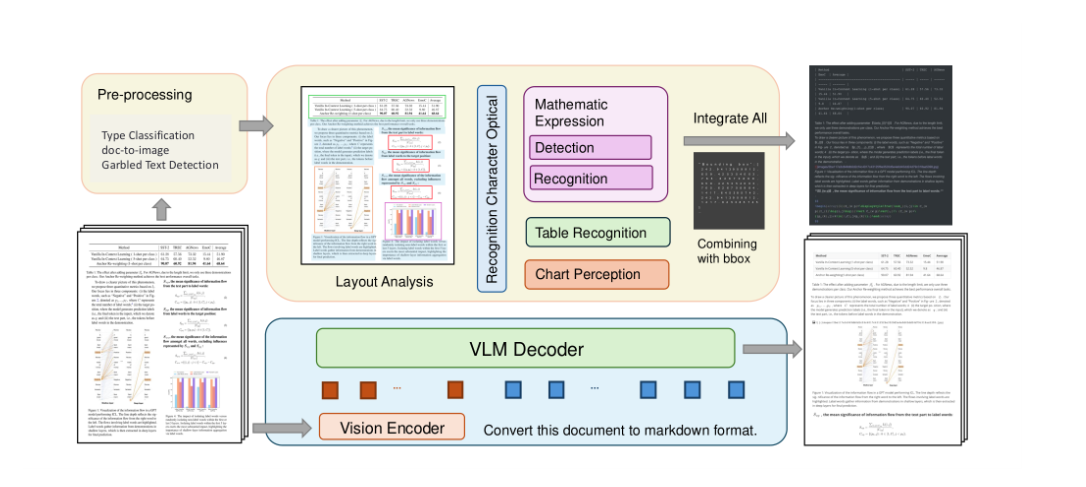
\includegraphics[scale=.6]{chapters/fig/template_matching_process.png}
    \caption{\it Processus de Template Matching : comparaison spatiale entre documents et templates}
    \cite{lu2003document}
    \label{fig:template-matching}
\end{figure}

Lu et Tan \cite{lu2003document} ont introduit une méthode basée sur les projections de blocs composants (\textit{Component Block Projections} CBP). Cette approche encode les relations spatiales entre les blocs constitutifs d'un document sous forme de vecteurs de projection directionnels. L'algorithme CBP offre deux avantages majeurs : une meilleure représentation des relations spatiales inter-blocs permettant une précision élevée même sur des images fortement déformées, et une réduction significative du coût computationnel grâce à l'exploitation de l'inégalité triangulaire \cite{lu2001document}.
\\
\textbf{Avantages} :
\begin{itemize}[label=\ding{42}, font=\large \color{darkgray}]
\item Précision exceptionnelle ($>$98\%) pour les documents à mise en page cohérente et prédéfinie.
\item Résultats déterministes et prédictibles, essentiels pour la conformité réglementaire.
\item Temps de traitement très rapide ($<$1 seconde par document).
\item Transparence totale de la logique d'extraction, facilitant le débogage et la validation.
\end{itemize}

\textbf{Inconvénients} :
\begin{itemize}[label=\ding{42}, font=\large \color{darkgray}]
\item \textbf{Sensibilité extrême aux variations de mise en page} : échec complet lorsque la structure du document dévie du modèle prédéfini.
\item \textbf{Scalabilité limitée} : la création manuelle d'un template pour chaque type de document engendre des coûts prohibitifs.
\item \textbf{Absence de capacité d'apprentissage} : tout nouveau format nécessite une reconfiguration intégrale plutôt qu'une adaptation incrémentale.
\end{itemize}


\subsubsection{Template Matching par descripteurs invariants}

Yang et al. \cite{yang2019hybrid} ont proposé une méthode hybride combinant caractéristiques locales et globales pour la reconnaissance de templates documentaires. Liu et al. \cite{liu2019sift} ont introduit une approche basée sur les descripteurs SIFT (\textit{Scale-Invariant Feature Transform}), invariants aux changements d'échelle et de rotation. Alnuaimi et al. \cite{alnuaimi2024similar} ont récemment proposé un algorithme de correspondance de templates similaires exploitant des réseaux de neurones convolutifs pour l'analyse de la mise en page documentaire, combinés à des réseaux récurrents pour la modélisation des dépendances séquentielles dans les documents à forte composante textuelle.
\\
\textbf{Avantages} :
\begin{itemize}[label=\ding{42}, font=\large \color{darkgray}]
\item Robustesse aux transformations géométriques (rotation, mise à l'échelle).
\item Meilleure tolérance aux déformations mineures du document.
\end{itemize}

\textbf{Inconvénients} :
\begin{itemize}[label=\ding{42}, font=\large \color{darkgray}]
\item \textbf{Coût computationnel élevé} dû à la combinaison de caractéristiques multiples.
\item \textbf{Complexité accrue} pour les ensembles de templates volumineux.
\end{itemize}


\subsubsection{Template Matching par graphes}

Riba et al. \cite{riba2022table} ont proposé une approche par graphes neuronaux pour la détection de tableaux dans les documents de facturation. Cette méthode modélise les relations structurelles entre les éléments d'un document sous forme de graphe, permettant une correspondance plus flexible que les approches purement spatiales.
\\
\textbf{Avantages} :
\begin{itemize}[label=\ding{42}, font=\large \color{darkgray}]
\item Représentation riche des relations structurelles entre éléments documentaires.
\item Flexibilité accrue pour les documents à structure variable.
\end{itemize}

\textbf{Inconvénients} :
\begin{itemize}[label=\ding{42}, font=\large \color{darkgray}]
\item \textbf{Coût computationnel prohibitif} pour les graphes de grande taille.
\item \textbf{Complexité d'implémentation} nécessitant une expertise en théorie des graphes.
\end{itemize}


\subsection{Extraction documentaire par OCR}

La Reconnaissance Optique de Caractères (\textit{Optical Character Recognition} OCR) constitue la méthode la plus polyvalente pour convertir les images de documents en texte exploitable. Les moteurs OCR modernes exploitent des réseaux neuronaux de type LSTM pour améliorer la précision de reconnaissance.

\subsubsection{Moteurs OCR open-source}

La figure~\ref{fig:ocr-pipeline} montre le pipeline complet de traitement OCR, incluant la détection de texte, la reconnaissance de caractères et la génération de sortie structurée.

\begin{figure}[H]
    \centering
    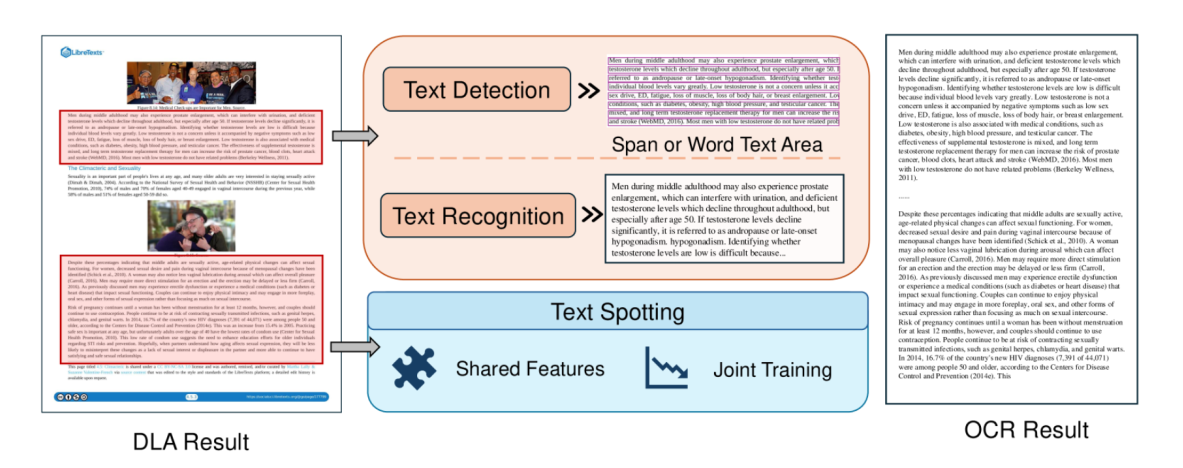
\includegraphics[scale=.6]{chapters/fig/ocr_pipeline.png}
    \caption{\it Pipeline OCR : détection de texte, reconnaissance et sortie structurée}
    \cite{du2022ppocr}
    \label{fig:ocr-pipeline}
\end{figure}

\textbf{Tesseract} \cite{smith2007tesseract}, maintenu par Google depuis 2006, est le moteur OCR open-source le plus largement adopté. Sa version 5.5.3 intègre un moteur de reconnaissance basé sur les réseaux LSTM, offrant une précision significativement supérieure aux versions précédentes sur les documents imprimés standards. Un benchmark de 2024 a montré que Tesseract atteint une précision de 92\% sur le texte anglais imprimé, avec un temps de traitement d'environ 453 ms par page \cite{webpii2025benchmark}.

\textbf{PaddleOCR} \cite{du2022ppocr}, développé par Baidu, offre une analyse de layout intégrée via son module PP-StructureV3, particulièrement adapté au traitement de tableaux et de documents multilingues. Sa précision atteint 93\% mais au prix d'une latence plus élevée (2143 ms).

\textbf{EasyOCR} \cite{jaidedai2024easyocr}, développé par Jaided AI, se distingue par sa prise en charge de l'écriture manuscrite et des documents à scripts mixtes, supportant plus de 80 langues avec une architecture légère et facile à intégrer.
\\
\textbf{Avantages} :
\begin{itemize}[label=\ding{42}, font=\large \color{darkgray}]
\item Flexibilité élevée face à la diversité des mises en page documentaires.
\item Fonctionnement sans pré-configuration sur la plupart des types de documents.
\item Précision raisonnable (90--95\%) sur les documents standards.
\item Bonne scalabilité en volume avec des performances consistantes.
\end{itemize}

\textbf{Inconvénients} :
\begin{itemize}[label=\ding{42}, font=\large \color{darkgray}]
\item \textbf{Perte des relations spatiales critiques} entre les éléments textuels, problématique pour le traitement des tableaux où l'alignement des colonnes est essentiel.
\item \textbf{Complexité des règles post-traitement} croissant exponentiellement avec la diversité documentaire.
\item \textbf{Dégradation significative} (20--30\%) sur les images de mauvaise qualité.
\item \textbf{Absence de compréhension sémantique} : extraction de texte sans appréhension du contexte métier.
\end{itemize}


\subsubsection{Plateformes cloud d'extraction documentaire}

Les grands fournisseurs cloud proposent des services managés combinant OCR et intelligence artificielle. Un benchmark indépendant (DeltOCR Bench, novembre 2025) a évalué ces services sur des types de documents mixtes et a placé Azure Document Intelligence en tête avec une précision d'environ 96\% sur le texte imprimé \cite{hegghammer2022ocr}.

\textbf{AWS Textract} \cite{aws2024textract} extrait le texte imprimé, l'écriture manuscrite, les tableaux, les formulaires et les paires clé-valeur via cinq API distinctes. Son avantage principal réside dans l'intégration native avec l'écosystème AWS (S3, Lambda, Step Functions).

\textbf{Azure Document Intelligence} \cite{microsoft2024azure} (anciennement Form Recognizer) offre la meilleure précision benchmark ($\sim$96\%) et un support fort pour les formulaires et factures, intégré à l'écosystème Microsoft Foundry.

\textbf{Google Document AI} \cite{google2024documentai} propose un écosystème de processeurs spécialisés (factures, contrats, ID) avec une intégration dans Vertex AI et BigQuery.

La figure~\ref{fig:cost-comparison} présente la comparaison des coûts en fonction du volume de documents traités pour les trois plateformes principales.

\begin{figure}[H]
    \centering
    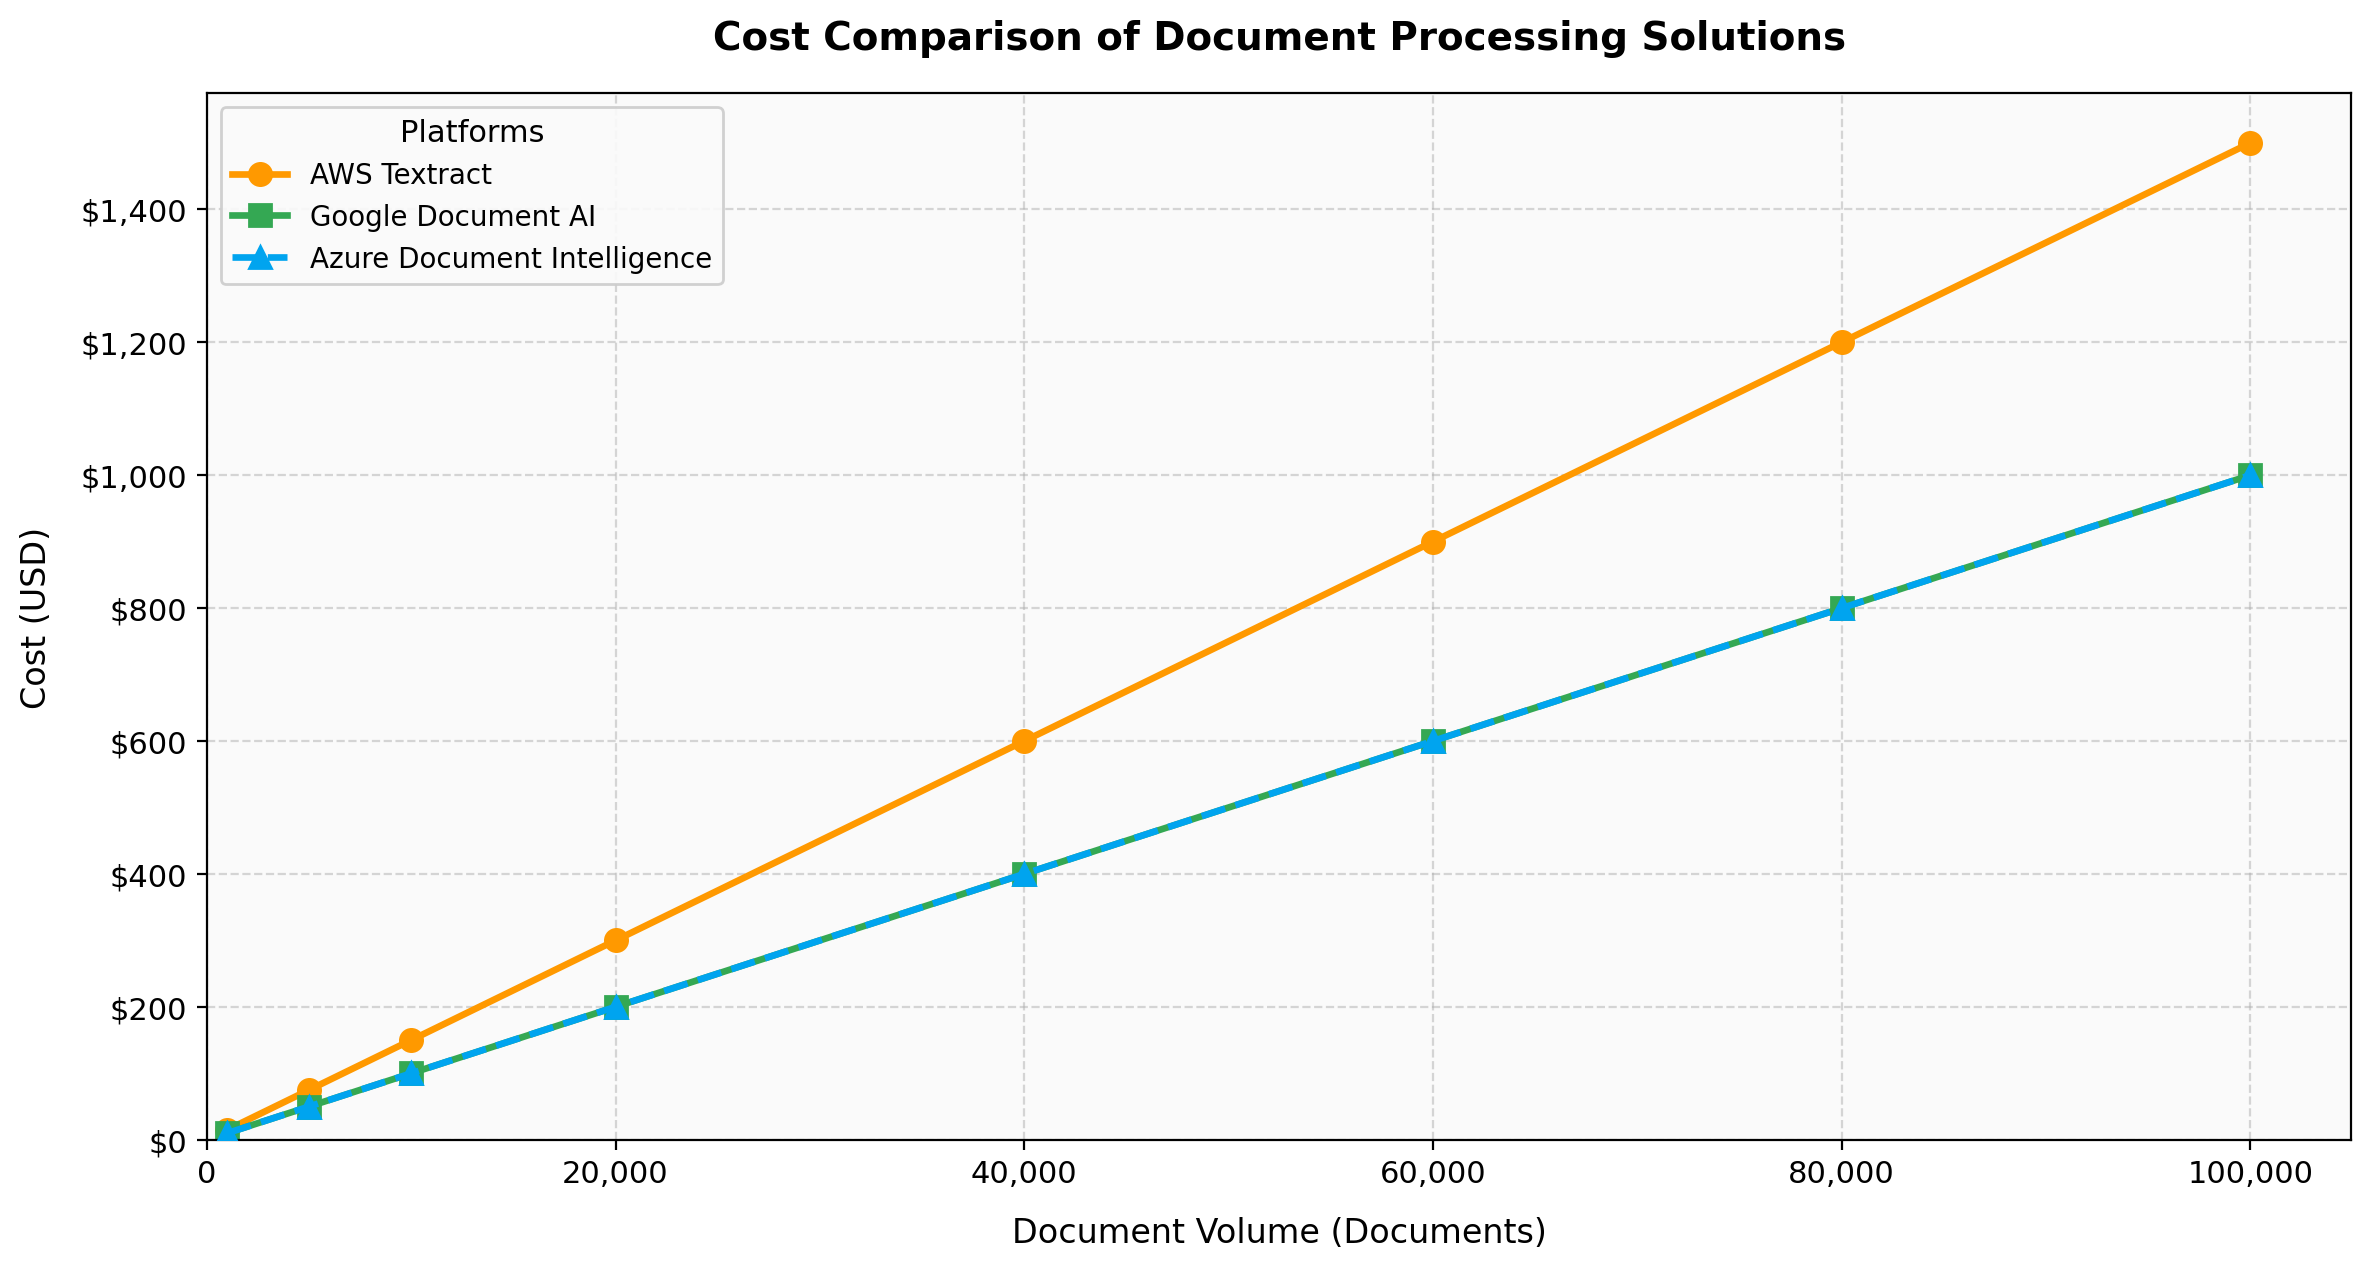
\includegraphics[scale=.6]{chapters/fig/cost_comparison.png}
    \caption{\it Comparaison des coûts des plateformes cloud en fonction du volume documentaire}
    \label{fig:cost-comparison}
\end{figure}


\subsection{Extraction documentaire par apprentissage automatique et IA}

Les approches par IA représentent l'évolution la plus récente du domaine, traitant les documents de manière end-to-end en combinant compréhension visuelle et analyse sémantique.

\subsubsection{Architectures Transformer pour la compréhension documentaire}

Les architectures Transformer ont révolutionné la compréhension documentaire en intégrant simultanément le texte, la mise en page et les informations visuelles. La famille LayoutLM, initiée par Xu et al. \cite{xu2020layoutlm}, constitue l'avancée la plus significative dans ce domaine.

La figure~\ref{fig:layoutlm-evolution} présente l'évolution des architectures de compréhension documentaire, des systèmes modulaires à base de templates vers les approches end-to-end modernes.

\begin{figure}[H]
    \centering
    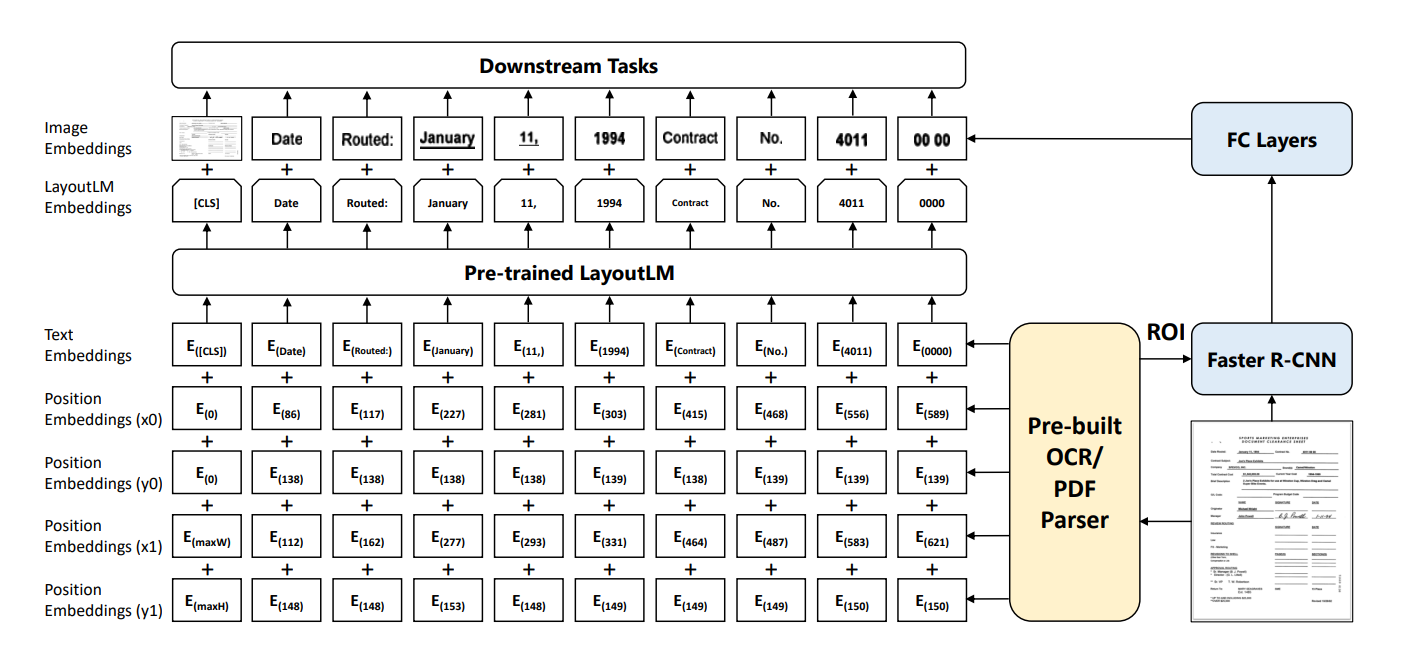
\includegraphics[scale=.6]{chapters/fig/ai_document_evolution.png}
    \caption{\it Évolution des systèmes d'extraction : du template matching aux approches end-to-end par IA}
    \cite{du2022ppocr}
    \label{fig:layoutlm-evolution}
\end{figure}

\textbf{LayoutLM} \cite{xu2020layoutlm} a introduit la modélisation conjointe du texte et des embeddings de position 2D, permettant au modèle de comprendre la relation entre le contenu textuel et sa position spatiale dans le document. Ce modèle a été pré-entraîné sur plus de 11 millions de pages de documents.

\textbf{LayoutLMv2} \cite{xu2021layoutlmv2} a étendu ce paradigme en incorporant des caractéristiques visuelles pour améliorer l'alignement cross-modal dans les documents visuellement riches. Le pré-entraînement multimodal combine trois types d'information : le texte tokenisé, les coordonnées des boîtes englobantes, et les patches visuels extraits par un encodeur d'image.

\textbf{LayoutLMv3} \cite{huang2022layoutlmv3} a unifié le masking du texte et des images lors du pré-entraînement, éliminant le besoin de détecteurs d'objets pré-entraînés et utilisant des couches linéaires comme extracteurs de caractéristiques visuelles, apportant ainsi une meilleure flexibilité.

D'autres architectures notables méritent d'être mentionnées :
\begin{itemize}[label=\ding{42}, font=\large \color{darkgray}]
\item \textbf{DocFormer} \cite{appalaraju2021docformer} : unifie les représentations textuelles, spatiales et visuelles dans une architecture end-to-end intégrée.
\item \textbf{LiLT} (\textit{Language-Independent Layout Transformer}) \cite{wang2022lilt} : propose un découplage des flux textuels et spatiaux avec un mécanisme d'attention bidirectionnel complémentaire, permettant le transfert cross-lingue zero-shot.
\item \textbf{DocLLM} \cite{wang2024docllm} : conditionne les modèles de langage génératifs sur les embeddings de boîtes englobantes pour produire du texte structuré respectant la mise en page documentaire, sans encodeur visuel lourd.
\end{itemize}


\subsubsection{Reconnaissance d'entités nommées (NER) pour l'extraction documentaire}

La Reconnaissance d'Entités Nommées (\textit{Named Entity Recognition}  NER) constitue un composant essentiel de l'extraction d'informations. Le NER identifie et classifie les mentions d'entités dans le texte en catégories prédéfinies telles que les noms de personnes (PER), les organisations (ORG), les lieux (LOC), les dates et les montants \cite{li2022survey}.

Dans le contexte de l'extraction documentaire, le NER est particulièrement utile pour :
\begin{itemize}[label=\ding{42}, font=\large \color{darkgray}]
\item L'identification automatique des champs clés dans les factures (montants, dates, numéros de référence).
\item L'extraction des informations personnelles dans les CV (nom, adresse, expérience professionnelle).
\item La détection des entités juridiques dans les documents administratifs (KBIS, RIB).
\end{itemize}

Les approches récentes exploitent des modèles pré-entraînés tels que BERT \cite{devlin2019bert} et ses variantes, atteignant des scores F1 supérieurs à 91\% sur les benchmarks standards \cite{li2022survey}. L'intégration du NER avec les modèles de compréhension documentaire (LayoutLM + NER) permet d'exploiter simultanément le contexte textuel et spatial pour une extraction plus précise des entités dans les documents structurés.
\\
\textbf{Avantages} :
\begin{itemize}[label=\ding{42}, font=\large \color{darkgray}]
\item Compréhension sémantique sophistiquée avec des performances consistantes (90--95\%) sur des layouts complexes et variés.
\item Adaptabilité supérieure aux nouveaux formats grâce à l'apprentissage par transfert.
\item Capacité d'apprentissage à partir d'exemples plutôt que par programmation explicite.
\end{itemize}

\textbf{Inconvénients} :
\begin{itemize}[label=\ding{42}, font=\large \color{darkgray}]
\item \textbf{Exigences massives en données d'entraînement} : des milliers d'exemples annotés par type de document et des ressources GPU substantielles.
\item \textbf{Nature boîte noire} : défis d'interprétabilité critiques pour la conformité réglementaire.
\item \textbf{Temps de développement extensif} : semaines à mois pour l'entraînement et le réglage fin.
\item \textbf{Sacrifice de la précision numérique} pour la compréhension sémantique, problématique pour les documents financiers.
\end{itemize}


\newpage
\section{État de l'Art}

Dans cette section, nous passons en revue les solutions existantes afin d'en dégager les avantages et limites de chacune d'elles.

\subsection{AWS Textract (Amazon)}
\textbf{Description} :
AWS Textract est un service cloud développé par Amazon Web Services pour l'extraction automatique de texte, de formulaires, de tableaux et de paires clé-valeur à partir de documents numérisés ou natifs. Il propose cinq API distinctes : Detect Document Text, Analyze Document (Forms/Tables/Queries/Signatures), Analyze Expense, Analyze ID et Analyze Lending \cite{aws2024textract}.

La figure~\ref{fig:textract-arch} présente l'architecture fonctionnelle d'AWS Textract.
\begin{figure}[htbp]
    \centering
    \resizebox{\linewidth}{!}{%
        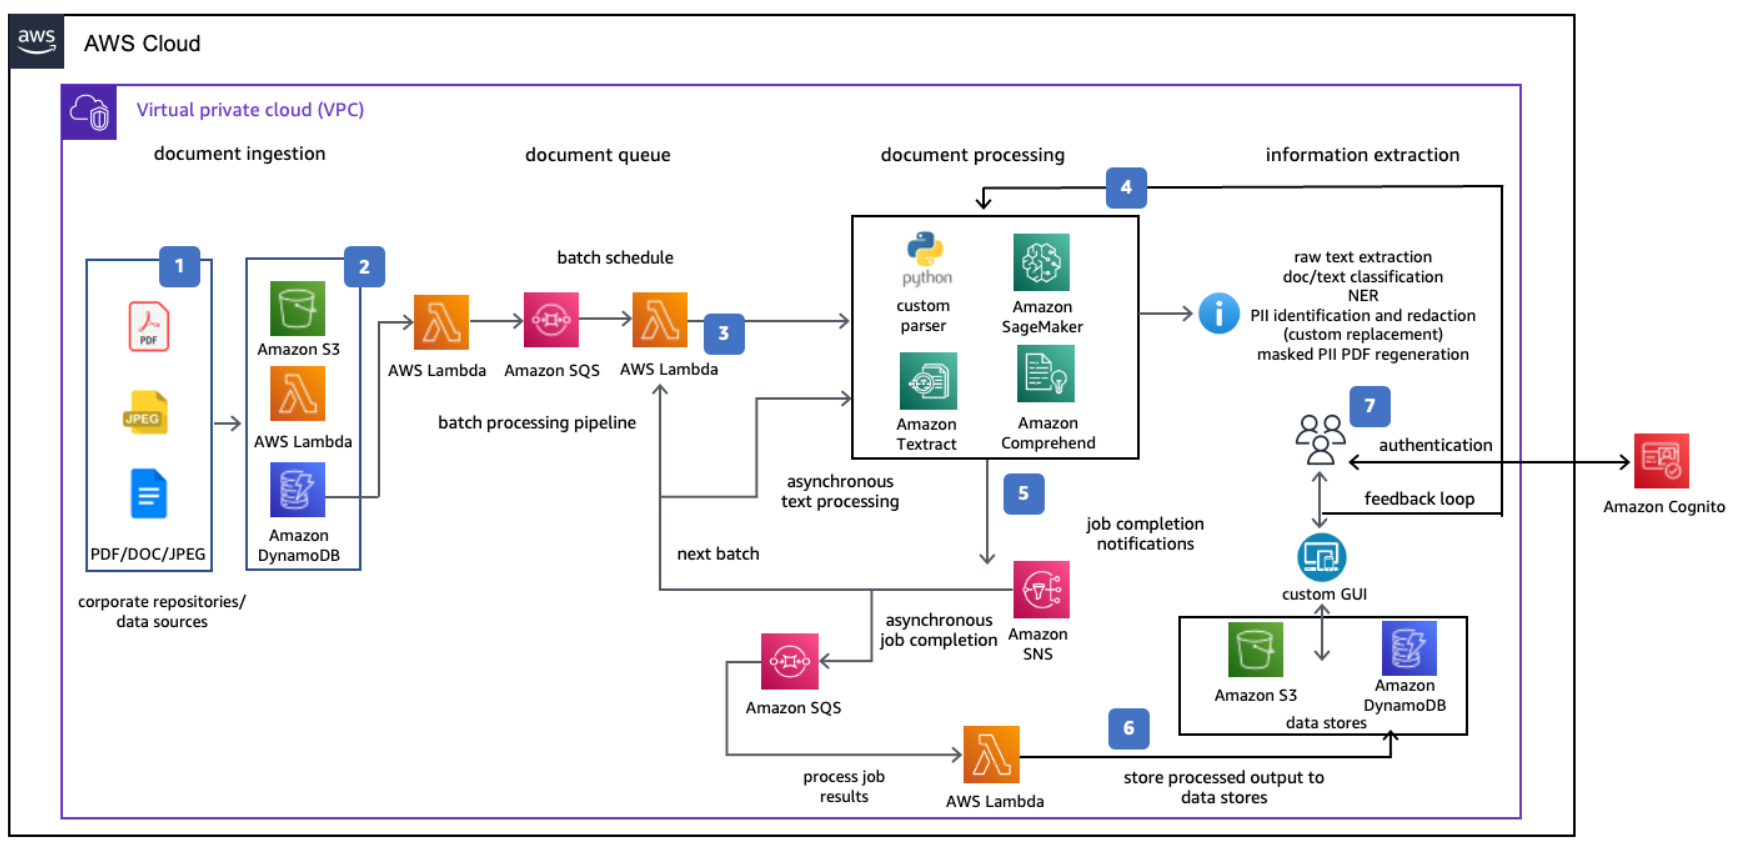
\includegraphics{chapters/fig/aws_textract_architecture.png}%
    }
    \caption{\itshape Architecture fonctionnelle AWS Textract}
    \cite{aws2024textract}
    \label{fig:textract-arch}
\end{figure}

L'architecture repose sur des modèles de deep learning pré-entraînés capables de détecter et d'extraire des informations structurées. Pour les factures, l'API AnalyzeExpense identifie automatiquement les champs métier standards (fournisseur, montant, date, lignes de facturation) sans configuration de templates.
\\
\textbf{Avantages} :
\begin{itemize}[label=\ding{42}, font=\large \color{darkgray}]
\item \textbf{Intégration native AWS} : connexion directe avec S3, Lambda et Step Functions pour des pipelines d'extraction automatisés.
\item \textbf{Précision compétitive} : $\sim$95\% sur le texte imprimé standard.
\item \textbf{Extraction de tableaux robuste} : capacité à préserver la structure tabulaire des documents.
\item \textbf{Scalabilité} : traitement de volumes importants sans gestion d'infrastructure.
\end{itemize}

\textbf{Inconvénients} :
\begin{itemize}[label=\ding{42}, font=\large \color{darkgray}]
\item \textbf{Tarification complexe} : facturation séparée par fonctionnalité (OCR basique : \$1,50/1000 pages ; avec tableaux : \$15/1000 pages ; avec formulaires : \$50/1000 pages).
\item \textbf{Dépendance cloud} : traitement exclusivement en ligne, impossibilité de déploiement on-premise.
\item \textbf{Dégradation sur scans de mauvaise qualité} : précision chutant à $\sim$76\% sur les documents dégradés.
\end{itemize}


\subsection{Azure Document Intelligence (Microsoft)}
\textbf{Description} :
Azure Document Intelligence (anciennement Form Recognizer) est le service d'extraction documentaire de Microsoft, intégré à l'écosystème Azure Foundry. Il offre des modèles pré-entraînés pour les factures, reçus, documents d'identité et contrats, avec la possibilité de créer des modèles personnalisés \cite{microsoft2024azure}.
La figure~\ref{fig:azure-arch} présente l'architecture d'Azure Document Intelligence.
\begin{figure}[H]
    \centering
    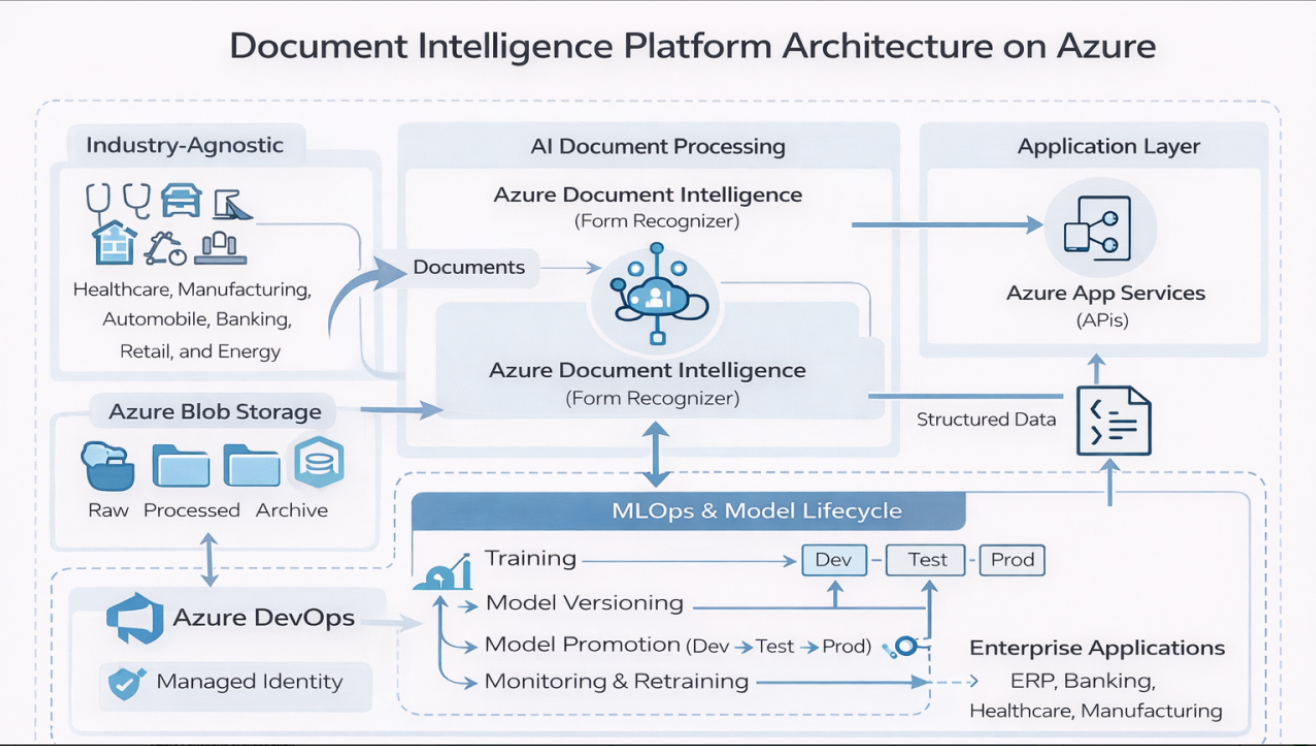
\includegraphics[scale=.6]{chapters/fig/azure_document_intelligence.png}
    \caption{\it Architecture Azure Document Intelligence}
    \cite{microsoft2024azure}
    \label{fig:azure-arch}
\end{figure}

\textbf{Avantages} :
\begin{itemize}[label=\ding{42}, font=\large \color{darkgray}]
\item \textbf{Meilleure précision benchmark} : $\sim$96\% sur le texte imprimé (DeltOCR Bench, novembre 2025).
\item \textbf{Support formulaires avancé} : extraction précise des paires clé-valeur et des structures tabulaires complexes.
\item \textbf{Intégration Microsoft} : connexion native avec Power Automate, Dynamics 365 et Azure Foundry.
\item \textbf{Déploiement hybride} : possibilité de conteneurs pour un traitement on-premise.
\end{itemize}

\textbf{Inconvénients} :
\begin{itemize}[label=\ding{42}, font=\large \color{darkgray}]
\item \textbf{Documentation fragmentée} : répartie entre Azure Foundry, AI Services et l'ancien Cognitive Services.
\item \textbf{Coût élevé pour l'extraction structurée} : \$10--50/1000 pages selon les fonctionnalités.
\item \textbf{Verrouillage écosystème} : intégration optimale uniquement dans l'environnement Microsoft.
\end{itemize}


\subsection{Google Document AI (Google)}
\textbf{Description} :
Google Document AI est la plateforme d'extraction documentaire de Google Cloud, proposant un écosystème de processeurs spécialisés pour différents types de documents (factures, contrats, documents d'identité). Elle s'intègre dans l'écosystème Vertex AI et BigQuery pour l'analyse downstream \cite{google2024documentai}.
\\
\textbf{Avantages} :
\begin{itemize}[label=\ding{42}, font=\large \color{darkgray}]
\item \textbf{Écosystème de processeurs riche} : processeurs spécialisés pré-entraînés pour de nombreux types documentaires.
\item \textbf{Précision compétitive} : $\sim$95\% sur le texte imprimé, avec des performances supérieures sur les pages denses.
\item \textbf{Intégration ML pipeline} : connexion directe avec Vertex AI pour l'entraînement de modèles personnalisés.
\item \textbf{Support Human-in-the-Loop} : workflow de revue humaine intégré.
\end{itemize}

\textbf{Inconvénients} :
\begin{itemize}[label=\ding{42}, font=\large \color{darkgray}]
\item \textbf{Confusion de nommage produit} : Cloud Vision API, Document AI et OCR On-Prem (arrêté en septembre 2025) sont des produits distincts souvent confondus.
\item \textbf{Verrouillage GCP} : dépendance à l'écosystème Google Cloud.
\item \textbf{Couverture linguistique} : performances variables selon les langues, en particulier pour les langues à faibles ressources.
\end{itemize}


\subsection{Tesseract OCR (Google)}
\textbf{Description} :
Tesseract est un moteur OCR open-source initialement développé chez Hewlett-Packard entre 1985 et 1994, maintenu par Google depuis 2006. La version 5.5.3 intègre un moteur de reconnaissance basé sur les réseaux LSTM, offrant des améliorations significatives de précision par rapport aux versions précédentes \cite{smith2007tesseract}.
\\
\textbf{Avantages} :
\begin{itemize}[label=\ding{42}, font=\large \color{darkgray}]
\item \textbf{Gratuit et open-source} : licence Apache 2.0, communauté active et documentation abondante.
\item \textbf{Support multilingue extensif} : plus de 100 langues supportées.
\item \textbf{Meilleur ratio précision/vitesse} : 92\% de précision avec 453 ms de latence par page.
\item \textbf{Intégration facile} : compatible avec Python (pytesseract), Java, C++ et de nombreux autres langages.
\end{itemize}

\textbf{Inconvénients} :
\begin{itemize}[label=\ding{42}, font=\large \color{darkgray}]
\item \textbf{Sensibilité à la qualité d'image} : performances dégradées sur les images bruitées et les scans de basse qualité.
\item \textbf{Absence de compréhension structurelle} : pas de détection native de la structure documentaire.
\item \textbf{Pré-traitement nécessaire} : requiert souvent une binarisation, un redressement et un débruitage en amont.
\item \textbf{Écriture manuscrite limitée} : performances faibles sur les annotations manuscrites.
\end{itemize}


\subsection{LayoutLM (Microsoft)}
\textbf{Description} :
LayoutLM est une famille de modèles Transformer pré-entraînés pour la compréhension de documents, développée par Microsoft Research. Ces modèles intègrent simultanément les informations textuelles, spatiales et visuelles pour comprendre la structure et le contenu des documents \cite{xu2020layoutlm, xu2021layoutlmv2, huang2022layoutlmv3}.

La figure~\ref{fig:layoutlm-arch} présente l'architecture de LayoutLMv3.
\begin{figure}[H]
    \centering
    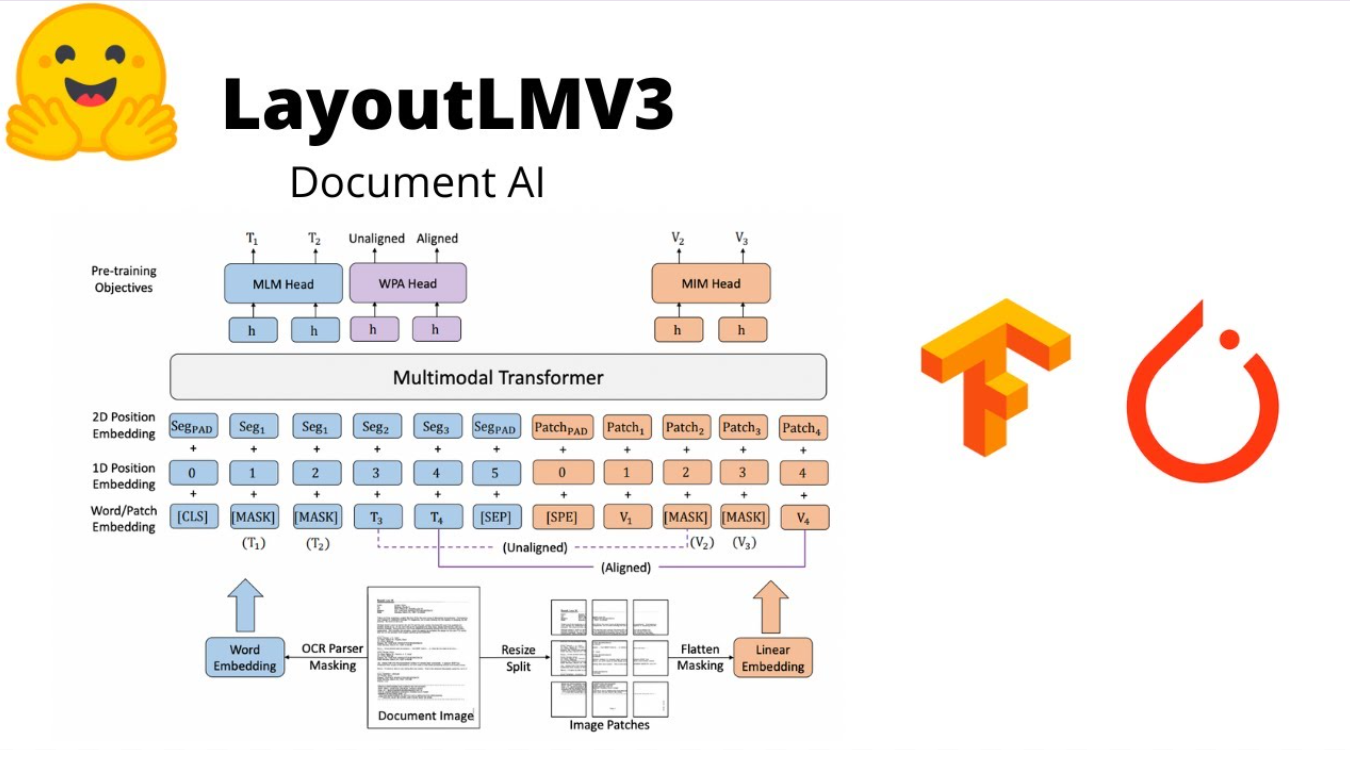
\includegraphics[scale=.6]{chapters/fig/layoutlmv3_architecture.png}
    \caption{\it Architecture LayoutLMv3 : pré-entraînement unifié texte et image}
    \cite{huang2022layoutlmv3}
    \label{fig:layoutlm-arch}
\end{figure}

\textbf{Avantages} :
\begin{itemize}[label=\ding{42}, font=\large \color{darkgray}]
\item \textbf{Compréhension multimodale} : intégration simultanée du texte, du layout et des informations visuelles.
\item \textbf{Performances état de l'art} : résultats supérieurs sur les benchmarks FUNSD, CORD et SROIE.
\item \textbf{Transfert d'apprentissage} : modèles pré-entraînés adaptables par fine-tuning avec peu de données.
\end{itemize}

\textbf{\textit{Inconvénients}} :
\begin{itemize}[label=\ding{42}, font=\large \color{darkgray}]
\item \textbf{Ressources computationnelles élevées} : nécessite des GPU pour l'entraînement et l'inférence.
\item \textbf{Licence restrictive} : LayoutLMv2 et v3 sous licences non commerciales ; seul v1 est MIT.
\item \textbf{Dépendance OCR} : nécessite un moteur OCR en amont pour la tokenisation du texte.
\item \textbf{Données d'entraînement volumineuses} : pré-entraîné sur 11 millions de pages.
\end{itemize}


\newpage
\section{Bilan et positionnement}

\subsection{Bilan}

\subsubsection{Synthèse comparative des plateformes d'extraction documentaire}
Le tableau~\ref{tab:platforms} présente un résumé comparatif des différentes plateformes d'extraction documentaire.

\begin{table}[H]
\centering
\caption{Tableau comparatif des plateformes d'extraction documentaire}
\resizebox{\textwidth}{!}{% 
\begin{tabular}{|l|l|l|l|l|l|}
\hline
\rowcolor[HTML]{FFCCCC}
\textbf{Critère} & \textbf{AWS Textract} & \textbf{Azure Doc. Intel.} & \textbf{Google Doc. AI} & \textbf{Tesseract 5.5.3} & \textbf{LayoutLMv3} \\ \hline
Précision (texte imprimé) & $\sim$95\% & $\sim$96\% & $\sim$95\% & $\sim$92\% & 90--95\% \\ \hline
Tarification & \$1,50--65/1k p. & \$1,50--50/1k p. & \$1,50--30/1k p. & Gratuit & Gratuit \\ \hline
Extraction tableaux & Excellente & Très bonne & Bonne & Limitée & Bonne \\ \hline
Extraction formulaires & Très bonne & Excellente & Bonne & Non supportée & Très bonne \\ \hline
Déploiement on-premise & Non & Oui (conteneurs) & Limité & Oui & Oui \\ \hline
Compréhension sémantique & Moyenne & Moyenne & Moyenne & Nulle & Élevée \\ \hline
Interprétabilité & Moyenne & Moyenne & Moyenne & Élevée & Faible \\ \hline
Écosystème & AWS & Microsoft & GCP & Indépendant & Indépendant \\ \hline
Support communautaire & Moyen & Moyen & Moyen & Élevé & Élevé \\ \hline
\end{tabular}
}
\label{tab:platforms}
\end{table}

Les plateformes actuelles d'extraction documentaire présentent plusieurs limites majeures :

\begin{enumerate}

\item \textbf{Compromis précision-flexibilité non résolu} :\\
Les systèmes à base de templates offrent une précision supérieure à 98\% mais échouent face aux variations de mise en page. Les systèmes d'IA offrent de la flexibilité mais requièrent des ressources considérables en données et en calcul. Aucune approche unique ne parvient à satisfaire simultanément ces deux exigences \cite{borchmann2021due}.

\item \textbf{Perte des relations spatiales par l'OCR} :\\
Les moteurs OCR extraient le texte de manière séquentielle, perdant les relations spatiales critiques entre les éléments. Cette limitation est particulièrement problématique pour le traitement des tableaux et des formulaires où l'alignement des colonnes est essentiel à l'interprétation des données.

\item \textbf{Écart laboratoire-production} :\\
Les benchmarks académiques utilisent des documents propres et à haute résolution, tandis que les environnements d'entreprise traitent des fax, des photos mobiles et des numérisations de qualité variable. Ces conditions réduisent la précision de 10 à 30\% par rapport aux conditions de test contrôlées \cite{hegghammer2022ocr}.

\item \textbf{Coût et complexité d'intégration} :\\
Les plateformes cloud facturent par page et par fonctionnalité, rendant les coûts imprévisibles à grande échelle. L'intégration avec les systèmes d'information d'entreprise nécessite un développement custom significatif.

\end{enumerate}


\subsubsection{Synthèse comparative des approches d'extraction}

Le tableau~\ref{tab:approaches} présente un résumé comparatif des trois grandes familles d'approches d'extraction documentaire.

\begin{table}[H]
    \centering
    \caption{Tableau comparatif des approches d'extraction documentaire}
    \begin{tabular}{|l|l|l|l|}
        \hline
        \rowcolor[HTML]{FFCCCC}
        \textbf{Critère} & \textbf{Template Matching} & \textbf{OCR} & \textbf{ML / IA} \\ \hline
        Précision & Très élevée ($>$98\%) & Moyenne (90--95\%) & Élevée (90--95\%) \\ \hline
        Flexibilité & Très faible & Élevée & Très élevée \\ \hline
        Temps de traitement & $<$1 s/doc & 1--5 s/doc & 2--10 s/doc \\ \hline
        Coût de déploiement & Faible & Moyen & Élevé (GPU) \\ \hline
        Adaptabilité & Nulle & Limitée & Forte \\ \hline
        Interprétabilité & Totale & Élevée & Faible \\ \hline
        Données requises & Templates manuels & Aucune & Milliers d'exemples \\ \hline
        Maintenance & Faible & Moyenne & Élevée \\ \hline
        Conformité & Excellente & Bonne & Difficile \\ \hline
    \end{tabular}
    \label{tab:approaches}
\end{table}

Cette classification illustre que, bien que les approches par IA dominent en termes de flexibilité et de compréhension sémantique, elles restent coûteuses et opaques. Les systèmes à base de templates sont très précis mais rigides. L'OCR offre un bon compromis mais perd les relations spatiales essentielles. Aucune approche isolée ne répond pleinement aux exigences d'un système d'extraction documentaire robuste et polyvalent.


\subsection{Positionnement}

Dans le Bilan précédent, nous avons vu que les plateformes actuelles d'extraction documentaire présentent chacune des forces et des faiblesses complémentaires. Plus loin, comme vu au tableau~\ref{tab:approaches}, le choix de l'approche d'extraction impacte directement la précision, la flexibilité et le coût du système, et est conditionné principalement par la diversité des types de documents à traiter, la disponibilité des ressources computationnelles et les exigences de conformité.

Au vu de tous ces paramètres, et de la réalité du terrain (documents d'entreprise variés, nécessité de précision élevée avec un coût maîtrisé), nous choisissons de développer un \textbf{framework hybride} qui s'appuiera sur :

\begin{itemize}[label=\ding{42}, font=\large \color{darkgray}]
\item Une \textbf{classification multi-modale} des documents permettant d'orienter dynamiquement le traitement vers la méthode d'extraction la plus appropriée.
\item La \textbf{préservation des relations spatiales} à travers des algorithmes de correspondance template fondés sur des vecteurs spatiaux.
\item L'\textbf{adaptation incrémentale des templates} via des mécanismes d'apprentissage qui permettent au système d'évoluer avec les corrections utilisateur.
\item Des \textbf{garanties mathématiques} de précision à travers une formalisation rigoureuse des coûts de commutation et des bornes d'erreur.
\end{itemize}

Ce nouveau cadre permettra de concilier la précision des systèmes à base de templates ($>$98\%), la flexibilité de l'OCR et la capacité d'adaptation de l'IA, tout en fournissant des garanties formelles de fiabilité pour le traitement documentaire en contexte d'entreprise.